\documentclass[10pt, letterpaper]{report}
% !TeX program = xelatex
%==================PREAMBOLO=======================%
\usepackage[utf8]{inputenc}
\usepackage{psvectorian}
\usepackage{pgfplots}
\usepackage[Rejne]{fncychap}
\usepackage[export]{adjustbox}
\usepackage[T1]{fontenc}
\usepackage{lmodern}
\usepackage[shortlabels]{enumitem}
\usepackage{moresize}
\usepackage{graphicx} % Required for inserting images
\usepackage{hyperref}
\usepackage{listings}
\usepackage[table,xcdraw]{xcolor}
\usepackage{amssymb}
\usepackage{amsmath}
\usepackage[italian]{babel}
\usepackage{nicefrac, xfrac}
\usepackage{tikz}
\usepackage{mathrsfs} 
\usepackage{titletoc}
\usepackage{fancyhdr}
\usepackage{psvectorian,lipsum}
\usepackage{fourier-orns}
\usepackage{lipsum}
\usepackage[paper=a4paper,left=25mm,right=25mm,bottom=25mm,top=25mm]{geometry}
\definecolor{light-gray}{gray}{0.95}
\definecolor{cop}{HTML}{f7ecd7}
\definecolor{copAut}{HTML}{ababab}
\definecolor{copAut2}{HTML}{c3c3e6}
\definecolor{purcop}{HTML}{d0d3db}
\definecolor{sapienza}{HTML}{660f1d}
\definecolor{lightSapienza}{HTML}{e3d3d5}
\definecolor{darkgreen}{HTML}{008000}
\definecolor{cartaRiciclata}{HTML}{fcfcf7}
\newcommand{\redText}[1]{\color{red}#1\color{black}}
\newcommand{\code}[1]{\colorbox{light-gray}{\texttt{#1}}}
\newcommand{\codee}[1]{\colorbox{white}{\texttt{#1}}}
\newcommand{\K}{{\mathbb K}}
\newcommand{\notimplies}{%
  \mathrel{{\ooalign{\hidewidth$\not\phantom{=}$\hidewidth\cr$\implies$}}}}
\newcommand{\flowerLine}{ \begin{center}\decofourleft\hphantom{ }\decoone\hphantom{ }\decofourright\hphantom{}\hphantom{aa}
\decofourleft\hphantom{ }\decoone\hphantom{ }\decofourright\hphantom{}\hphantom{aa}
\decofourleft\hphantom{ }\decoone\hphantom{ }\decofourright\hphantom{}\hphantom{aa}
\decofourleft\hphantom{ }\decoone\hphantom{ }\decofourright\hphantom{}\hphantom{aa} 
\decofourleft\hphantom{ }\decoone\hphantom{ }\decofourright\hphantom{}\hphantom{aa}
\decofourleft\hphantom{ }\decoone\hphantom{ }\decofourright\hphantom{}\hphantom{aa}
\decofourleft\hphantom{ }\decoone\hphantom{ }\decofourright\hphantom{}\hphantom{aa}
\decofourleft\hphantom{ }\decoone\hphantom{ }\decofourright\hphantom{}\hphantom{aa}
\decofourleft\hphantom{ }\decoone\hphantom{ }\decofourright\hphantom{}\hphantom{aa}
\end{center}}
\definecolor{g}{RGB}{60, 50, 50}
\newcommand{\textg}[1]{\color{g}{\textbf{#1}}\color{black}}
\newcommand{\teo}[1]{{\large\color{sapienza}\textbf{Teorema #1 :\hphantom{a}}}}
\newcommand{\defi}[1]{{\large\color{sapienza}\textbf{Definizione #1 :\hphantom{a}}}}
\newcommand{\claim}[1]{{\color{sapienza}\textbf{Claim #1 :\hphantom{a}}}}
\newcommand{\lemma}[1]{{\color{sapienza}\textbf{Lemma #1 :\hphantom{a}}}}
\newcommand{\dimo}[1]{{\color{sapienza}\textbf{Dimostrazione #1 :\hphantom{a}}}}
\newcommand{\prop}[1]{{\color{sapienza}\textbf{Proposizione #1 :\hphantom{a}}}}
\newcommand\greybox[1]{%
  \vskip\baselineskip%
  \par\noindent\colorbox{light-gray}{%
    \begin{minipage}{\textwidth}#1\end{minipage}%
  }%
  \vskip\baselineskip%
}
\newcommand\sapbox[1]{%
  \vskip\baselineskip%
  \par\noindent\colorbox{lightSapienza}{%
    \begin{minipage}{\textwidth}#1\end{minipage}%
  }%
  \vskip\baselineskip%
}

\newcommand{\Z}{{\mathbb Z}}
\newcommand{\blank}{{\sqcup}}
\newcommand{\R}{{\mathbb R}}
\newcommand{\N}{{\mathbb N}}
\newcommand{\C}{{\mathbb C}}
\newcommand{\Sn}{{\mathcal S_n}}
\newcommand{\An}{{\mathcal A_n}}
\newcommand{\E}{{\mathcal E}}
\newcommand{\B}{{\mathcal B}}
\newcommand{\mcm}{{\text{mcm}}}
\newcommand{\rg}{{\text{rg}}}
\newcommand{\ve}{{\bar v}}
\newcommand{\spaz}{{\text{\hphantom{aa}}}}
\newcommand{\MCD}{{\text{MCD}}}
\newcommand{\tc}{{\text{ tale che }}}
\newcommand{\supp}{{\text{Supp}}}
\newcommand{\acc}{\\\hphantom{}\\}
\newcommand{\aut}{{\text{Aut}}}
\newcommand{\Span}{{\text{Span}}}
\newcommand{\End}{{\text{End}}}
\newcommand{\cen}{{\text{Centro}}}
\newcommand{\norm}{{\unlhd}}
\newcommand{\ciclS}{{\left \langle }}
\newcommand{\ciclE}{{\right \rangle }}
\newcommand{\boxedMath}[1]{\begin{tabular}{|c|}\hline \texttt{#1} \\ \hline\end{tabular} :}
\newcommand{\shell}[1]{\colorbox{black}{\textcolor{white}{\texttt{#1}}}}
\newcommand{\eqImportante}[1]{\begin{center}\huge\lefthand\hphantom{a}
    \normalsize\texttt{#1}
    \hphantom{aaa}\huge\righthand\end{center}}

\fancyhf{}
\pagestyle{fancy}
\usepackage{pgf-pie}  
\usetikzlibrary{positioning}

\renewcommand{\headrule}{%
\vspace{-8pt}\hrulefill
\raisebox{-2.1pt}{\quad\decothreeleft\decotwo\decothreeright\quad}\hrulefill}

%sta roba serve per il codice C
\definecolor{mGreen}{rgb}{0,0.6,0}
\definecolor{mGray}{rgb}{0.5,0.5,0.5}
\definecolor{mPurple}{rgb}{0.58,0,0.82}
\definecolor{backgroundColour}{rgb}{0.95,0.95,0.92}

\lstdefinestyle{CStyle}{
    backgroundcolor=\color{backgroundColour},   
    commentstyle=\color{mGreen},
    keywordstyle=\color{magenta},
    numberstyle=\tiny\color{mGray},
    stringstyle=\color{mPurple},
    basicstyle=\footnotesize,
    breakatwhitespace=false,         
    breaklines=true,                 
    captionpos=b,                    
    keepspaces=true,                 
    numbers=left,                    
    numbersep=5pt,                  
    showspaces=false,                
    showstringspaces=false,
    showtabs=false,                  
    tabsize=2,
    language=C
}
\lstdefinestyle{CppStyle}{
    backgroundcolor=\color{backgroundColour},   
    commentstyle=\color{mGreen}\ttfamily,
    morecomment=[l][\color{magenta}]{\#}
    keywordstyle=\color{blue}\ttfamily,
    numberstyle=\tiny\color{mGray},
    stringstyle=\color{red}\ttfamily,
    basicstyle=\ttfamily,
    breakatwhitespace=false,         
    breaklines=true,                 
    captionpos=b,                    
    keepspaces=true,                 
    numbers=left,                    
    numbersep=5pt,                  
    showspaces=false,                
    showstringspaces=false,
    showtabs=false,                  
    tabsize=2,
    language=C
}
\lstset{language=C++,
                basicstyle=\ttfamily,
                keywordstyle=\color{blue}\ttfamily,
                stringstyle=\color{red}\ttfamily,
                commentstyle=\color{green}\ttfamily,
                morecomment=[l][\color{magenta}]{\#}
}
%fine roba che serve per il codice C
\usepackage{minted}
 %TOGLI COMMENTO SE USI XELATEX
%\usepackage{fontspec}
\title{Programmazione di Sistemi Multicore} %========TITOLO========%
\author{Marco Casu}
\date{\vspace{-5ex}}
\begin{document}

%==================COPERTINA=======================%
\begin{titlepage}
    \pagecolor{purcop}
\begin{center}
    %TOGLI COMMENTO SE USI XELATEX
   %\setmainfont{Palace Script MT}
   \Huge Marco Casu\acc
    %\setmainfont{Grand Casino}
     %TOGLI COMMENTO SE USI XELATEX
    %\setmainfont{h Halfroad}
    \HUGE \decothreeleft\hphantom{ }{\Huge\selectfont Programmazione di Sistemi Multicore}\hphantom{ }\decothreeright
     %TOGLI COMMENTO SE USI XELATEX
   % \setmainfont{Times New Roman}
\end{center}
\thispagestyle{empty}
\begin{figure}[h]
    \centering{
        %l'immagine deve avere una risoluzione 2048x2048
        
\includegraphics[width=1\textwidth ]{images/copertina.jpeg}
    }
\end{figure}
\vfill 
\centering 
\includegraphics[width=0.4\textwidth ]{../../preamble/Stemma_sapienza.png} \acc
\centering \Large \color{sapienza}Facoltà di Ingegneria dell'Informazione,
Informatica e Statistica\\
Dipartimento di Informatica
\end{titlepage}

%===================FINE COPERTINA======================%
\newpage
\pagecolor{cartaRiciclata}%\setmainfont{Algerian}
\large
Questo documento è distribuito sotto la licenza 
\color{blue}\href{https://www.gnu.org/licenses/fdl-1.3.txt}{GNU}\color{black},  
è un resoconto degli appunti (eventualmente integrati con libri di testo) tratti dalle lezioni del corso di Programmazione di Sistemi Multicore
\hphantom{a}per la laurea 
triennale in Informatica. Se dovessi notare errori, ti prego di segnalarmeli.
\vfill
\begin{figure}[h!]
    \raggedright
    
\includegraphics[width=0.4\textwidth,right ]{../../preamble/tomodachi.pdf} 
\end{figure}
\newpage %\setmainfont{Times New Roman}
\normalsize
\tableofcontents 
\newpage

%==================FOOTER e HEADER=======================%
\fancyhf{}
\fancyhead[L]{\nouppercase{\leftmark}}
\fancyhead[R]{Sezione \thesection}
\fancyfoot[C]{\thepage}
\fancyfoot[L]{Appunti di Prog. di Sistemi Multicore}
\fancyfoot[R]{ Marco Casu}
%\fancyfoot[R]{\setmainfont{Palace Script MT}\huge Marco Casu \setmainfont{Times New Roman}}
%==================FOOTER e HEADER=======================%

%Ricorda del comando \flowerLine per separare le sottosezioni. Le sezioni si separano nelle diverse pagine

%==================INIZIO======================%

\chapter{Parallelismo : Motivazioni}
\section{Introduzione}
In una \textit{GPU} (Graphics Processing Unit), nota anche come scheda video, ci sono circa 
80 miliardi di transistor, e vengono utilizzate per allenare i grossi modelli di intelligenza 
artificiale, i quali necessitano migliaia di GPU, non è un caso se \textit{Nvidia} ad oggi, con 
il boom dell'IA, è una delle aziende più quotate al mondo. Le GPU, e la loro 
programmazione, sono uno fra i principali argomenti di questo corso.\acc 
L'evoluzione dell'hardware, ha portato i grossi sistemi di computazione, ad essere formati da 
svariate unità di calcolo piuttosto che una singola unità molto potente, i processori stessi di uso comune, 
ad oggi sono composti da più \textit{core}.\acc 
La legge di Moore riguarda una stima empirica che mette in correlazione lo scorrere del tempo con 
l'aumentare della potenza di calcolo dei processori, se inizialmente, a partire dagli anni 70, tale potenza 
raddoppiava ogni due anni, ad oggi tale andamento è andato rallentando, raggiungendo un 
incremento 1.5 in 10 anni.
\begin{center}
    \includegraphics[width=300pt]{images/processor_trend.eps}
\end{center}
L'obbiettivo di costruire calcolatori sempre più potenti è dipeso dalla necessità dell'Uomo 
di risolvere problemi sempre più complessi, come ad esempio, la risoluzione del genoma umano.\acc 
Il motivo per il quale non è possibile costruire processori monolitici sempre più potenti, risiede 
in un \textit{limite fisico} riguardante la densità massima possibile dei transistor in 
un chip.\begin{enumerate}
    \item transistor più piccoli $\longrightarrow$ processori più veloci
    \item processori più veloci $\longrightarrow$ aumento del consumo energetico 
    \item aumento del consumo energetico $\longrightarrow$ aumento del calore 
    \item aumento del calore $\longrightarrow$ problemi di inaffidabilità dei transistor
\end{enumerate}
\flowerLine
\section{Modelli di Parallelismo}
L'informatico che intende scrivere del codice per un sistema multicore, deve esplicitamente 
sfruttare i diversi core, limitandosi a scrivere un codice sequenziale, non starebbe sfruttando a pieno 
l'hardware a disposizione, rendendo il processo meno efficiente di quanto potrebbe essere.\acc 
La maggior parte delle volte, un algoritmo sequenziale, non può essere direttamente tradotto in un 
algoritmo parallelo, per questo bisogna scrivere il codice facendo riferimento all'hardware di 
destinazione. Si consideri adesso il seguente codice sequenziale, che ha lo scopo di sommare 
$n$ numeri dati in input.
\begin{lstlisting}[style=CStyle]
    sum = 0;
    for(i=0; i<n; i++){
        x = compute_next_value(...);
        sum += x;
    }
\end{lstlisting}
Si vuole rendere tale algoritmo parallelo, sapendo di essere a disposizione di $p$ core.
\begin{lstlisting}[style=CStyle]
    local_sum = 0;
    first_index = ...;
    last_index = ...;
    for(local_i=first_index; first_index<last_index; local_i++){
        local_x = compute_next_value(...);
        local_sum += local_x;
    }
\end{lstlisting}
In tale esempio, ogni core possiede le sue variabili private non condivise con gli altri core, 
ed esegue indipendentemente il blocco di codice. Ogni core conterrà la somma
parziale di $\nicefrac{n}{p}$ valori.\acc 
\textbf{Esempio} (24 numeri, 8 core) :\begin{center}
    valori : $1,4,3,\;\;\;9,2,8,\;\;\;5,1,1,\;\;\;6,2,7,\;\;\;2,5,0,\;\;\;4,1,8,\;\;\;6,5,1,\;\;\;2,3,9$\acc 
    \begin{tabular}{|l|l|l|l|l|l|l|l|l|}
        \hline
        \rowcolor[HTML]{C0C0C0} 
        core & 0 & 1 & 2 & 3 & 4 & 5 & 6 & 7 \\ \hline
        \texttt{local\_sum}    & 8 & 19 & 7 & 15 & 7 & 13 & 12 & 14 \\ \hline
        \end{tabular}
\end{center}
A questo punto, per ottenere la somma totale, vi sarà un core \textit{master} che riceverà le somme 
parziali da tutti gli altri core, per poi eseguire la somma finale.
\begin{lstlisting}[style=CStyle]
    if(master){
        sum = local_sum;
        for c : core{
            if(c!=self){
                sum += c.local_sum;
            }
        }
    }else{
        send local_sum to master;
    }
\end{lstlisting}
Dividere i dati per poi far eseguire la stessa computazione ai diversi nodi è la forma più semplice 
di parallelismo. La soluzione adottata non è ideale, in quanto, in seguito al calcolo delle somme 
parziali, tutti i core escluso il master non staranno eseguendo calcoli. Una possibile 
idea alternativa è di far si che a coppie i nodi si condividano le somme parziali per poi calcolarne 
una somma comune, sviluppando uno scambio di dati ad albero, come mostrato in figura \ref{fig:tree_cores}.
\begin{figure}[h!]
    \centering
    \includegraphics[width=280pt]{images/tree.eps}
    \caption{calcolo somme a coppie}
    \label{fig:tree_cores}
\end{figure}\acc
Possiamo identificare due tipi di parallelismo :\begin{itemize}
    \item \textbf{parallelismo dei task} : fra i core vengono divise diverse attività che vengono 
    svolte autonomamente.
    \item \textbf{parallelismo dei dati} : i dati da elaborare vengono divisi, ogni core eseguirà 
    la stessa computazione ma su una porzione diversa dei dati.
\end{itemize}
Quando si scrive un programma parallelo bisogna prestare attenzione alla \textit{sincronizzazione} dei 
processi, in quanto potrebbero dover accedere ad una stessa area di memoria. Risulta cruciale 
saper mettere in \textit{comunicazione} i vari core, e suddividere equamente il 
\textit{carico di lavoro} fra di essi. Verranno considerate 4 diverse tecnologie per la programmazione 
multicore : \begin{itemize}
    \item \textit{MPI} (Message Passing Interface) [ libreria ]
    \item \textit{Posix} Threads [ libreria ]
    \item \textit{OpenMP} [ libreria e compilatore ]
    \item \textit{CUDA} [ libreria e compilatore ]
\end{itemize}
La programmazione delle GPU richiederà un diverso compilatore, e non il solito \texttt{gcc}, in quanto 
l'architettura della scheda video differisce da quella del processore, e con essa le istruzioni.\acc
I sistemi paralleli possono essere categorizzati sotto vari aspetti.\begin{itemize}
    \item \textbf{shared memory} : Tutti i core accedono ad un'area di memoria comune. L'accesso 
    e la sincronizzazione vanno gestiti con cautela.
    \item \textbf{distributed memory} : Ogni core ha un area di memoria privata, e la comunicazione 
    avviene attraverso un apposito canale per lo scambio dei messaggi. 
\end{itemize}
\begin{figure}[h!]
    \centering
    \includegraphics[width=280pt]{images/sdmem.eps}
    \caption{modelli di parallelismo}
    \label{fig:sdmem}
\end{figure}
Vi è un altra suddivisione nei sistemi paralleli :\begin{itemize}
    \item \textbf{MIMD} : Ogni core ha una control unit indipendente, diversi core possono eseguire 
    diverse istruzioni nello stesso momento.
    \item \textbf{SIMD} : Vi è un singolo program counter per tutti i core, che eseguono in maniera 
    parallela le stesse istruzioni. Due core non possono eseguire operazioni diverse nello stesso momento.
\end{itemize}
Le GPU hanno una struttura \textit{SIMD}.\begin{center}
    \begin{tabular}{c|
        >{\columncolor[HTML]{EFEFEF}}c |
        >{\columncolor[HTML]{EFEFEF}}c |}
        \cline{2-3}
                                                           & \cellcolor[HTML]{C0C0C0}shared memory & \cellcolor[HTML]{C0C0C0}distributed memory \\ \hline
        \multicolumn{1}{|c|}{\cellcolor[HTML]{C0C0C0}SIMD} & CUDA                                  &                                            \\ \hline
        \multicolumn{1}{|c|}{\cellcolor[HTML]{C0C0C0}MIMD} & Pthreads/OpenMP/CUDA                  & MPI                                        \\ \hline
        \end{tabular}
\end{center}
Fin'ora sono stati utilizzati 3 termini chiave riguardante i tipi di programmazione,
 sebbene non vi sia una definizione comunemente accettata, 
la seguente verrà adottata in tale contesto : \begin{itemize}
    \item \textit{concorrente} : più processi sono attivi in uno stesso momento 
    \item \textit{parallela} : diverse entità cooperative che operano in maniera ravvicinata per 
    un obbiettivo comune.
    \item \textit{distribuita} : diverse entità cooperative.
\end{itemize}
La programmazione parallela o distribuita implica che sia anche concorrente, non è vero il contrario.
\chapter{Memoria Distribuita : MPI}
\textit{MPI} è una libreria standard (avente varie implementazioni) necessaria allo sviluppo di codice multiprocesso 
a memoria distribuita. Precisamente, ogni core ha una memoria privata inaccessibile dall'esterno, e la comunicazione 
avviene attraverso una rete di interconnesione, (ad esempio, un bus), tale modello è detto \textbf{message 
passing}.
\section{La libreria OpenMpi}
Alla compilazione ed avvio di un programma che sfrutta MPI, ogni core eseguirà il programma, sarà la logica 
di esso a suddividere il carico di lavoro, tramite i costrutti decisionali. Verrà utilizzata un'implementazione 
nota come \textit{openMpi}, è possibile installare la libreria su sistemi operativi linux tramite il comando \acc
    \shell{sudo apt-get install libopenmpi-dev}
\acc
Il seguente esempio, mostra un programma che scrive sulla console una stringa, e tramite MPI, tale processo è avviato 
su ogni core.
\begin{lstlisting}[style=CStyle]
    #include <stdio.h>
    #include <mpi.h>
    //voglio lanciare il programma su piu unita di calcolo
    int main(int argc, char **argv){
        int p = MPI_Init(NULL,NULL); 
        //Il parametro in output di MPI_Init e' uno status sull'errore
        if(p == MPI_SUCCESS){
        
        }else{
            printf("qualcosa e' andato storto");
            MPI_Abort(MPI_COMM_WORLD,p);
            //Con MPI_Abort tutti i processi su tutti i core avviati verranno terminati 
        }
        printf("hello world");
        MPI_Finalize(); //Serve per terminare la libreria
        return 0;
    }
\end{lstlisting}
I programmi MPI non vengono compilati con \shell{gcc}, ma con \shell{mpicc}\acc 
\shell{mpicc hello\_world.c -o hello\_world.out}
\acc
Una volta ottenuto l'eseguibile, è possibile lanciare il programma con \shell{mpirun} specificando 
il numero di core sulla quale verrà eseguito il programma, tale numero, se non specificato con apposite flag, 
deve essere minore o uguale al numero di core fisici presenti sulla macchina.\acc 
\shell{mpirun -n 4 hello\_world.out}
\acc 
Ogni funzione della libreria ha una dicitura che inizia con \textit{"MPI\_"}. Ogni funzione di libreria deve essere chiamata 
fra \begin{itemize}
    \item \code{MPI\_Init} - configurazione ed avviamento della libreria 
    \item \code{MPI\_Finalize} - chiusura e deallocazione della memoria 
\end{itemize}
Tali righe stabiliscono il blocco di codice in cui verranno eseguite funzioni MPI.
\flowerLine 
\section{Rank e Comunicazione}
Ogni processo MPI è univocamente identificato da un numero intero detto \textit{rank}, se $p$ processi sono 
attivi, avranno gli identificatori $1,2\dots,p-1$.\acc  Un \textbf{comunicatore} è un insieme di processi, i quali hanno 
la possibilità di scambiarsi messaggi, si può pensare ad un comunicatore come un etichetta, e processi con la stessa 
etichetta possono comunicare fra loro. 
È identificabile nel codice tramite la struttura dati \code{MPI\_Comm}, e all'avvio di MPI, viene sempre 
definito un comunicatore di default \code{MPI\_COMM\_WORLD} che contiene tutti i processi.\acc 
L'identificatore di ogni processo è in realtà relativo ad ogni comunicatore, due processi diversi possono condividere il 
rank se relativo a comunicatori diversi. Ci sono due funzioni importanti che riguardano questi ultimi\begin{itemize}
    \item \code{int MPI\_Comm\_rank(MPI\_Comm comm, int *rank)} : Prende in input un comunicatore ed un numero intero, e 
    salva dentro tale numero il rank del processo chiamante relativo al comunicatore dato.
    \item \code{int MPI\_Comm\_size(MPI\_Comm comm, int *size)} : Prende in input un comunicatore ed un numero intero, e 
    salva dentro tale intero il numero di processi all'interno del comunicatore.
\end{itemize}
\begin{lstlisting}[style=CStyle]
    #include <stdio.h>
    #include <mpi.h>
    //voglio lanciare il programma su piu unita di calcolo
    int main(int argc, char **argv){
        int p = MPI_Init(NULL,NULL); 
        //Il parametro in output di MPI_Init e' uno status sull'errore
        if(p == MPI_SUCCESS){
        
        }else{
            printf("qualcosa e' andato storto");
            MPI_Abort(MPI_COMM_WORLD,p);
            //Con MPI_Abort tutti i processi su tutti i core avviati verranno terminati 
        }
        int size;
        MPI_Comm_size(MPI_COMM_WORLD, &size);
        int rank;
        MPI_Comm_rank(MPI_COMM_WORLD, &rank);
        printf("hello world, im the process %d/%d",rank,size);
        MPI_Finalize(); //Serve per terminare la libreria
        return 0;
    }
\end{lstlisting}
La comunicazione avviene tramite due funzioni, il cui comportamento è simile alla comunicazione tramite \code{pipe}.\acc 
L'inzio dei messagi avviene tramite \code{int MPI\_Send}, i cui parametri sono\begin{itemize}
    \item \code{void* msg\_buf\_p} l'area di memoria da trasferire al processo destinatario 
    \item \code{int msg\_size} il numero di elementi (non l'occupazione in byte) del messaggio da trasferire 
    \item \code{MPI\_Datatype msg\_type} il tipo di elemento da trasferire. Sono definiti dei tipi standard che 
    incorporano tutti i tipi più comuni del \textit{C}
    \item \code{int dest} il rank del processo destinatario
    \item \code{int tag} un tag da dare al messaggio per identificarlo 
    \item \code{MPI\_Comm communicator} il comunicatore  su cui avviene la comunicazione
\end{itemize}
Può dipendere dall'implementazione, ma solitamente quando un processo fa una \code{MPI\_Send}, si arresta finché 
il messaggio inviato non viene ricevuto dal destinatario, allo stesso modo, un destinatario che si appresta a ricevere 
un messaggio viene arrestato fino al ricevimento. Le chiamate di comunicazione MPI sono quindi bloccanti. \acc 
Per ricevere dati, viene utilizzata la chiamata \code{MPI\_Recv}  i cui parametri sono\begin{itemize}
    \item \code{void* msg\_buf\_p} l'area di memoria su cui verrà salvato il messaggio 
    \item \code{int buf\_size} il numero di elementi (non l'occupazione in byte) del messaggio da ricevere 
    \item  \code{MPI\_Datatype buf\_type} il tipo di elemento da ricevere
    \item \code{int source} il rank del processo mittente
    \item \code{int tag} il tag del messaggio da ricevere
    \item \code{MPI\_Comm communicator} il comunicatore su cui avviene la comunicazione
    \item \code{MPI\_Status* status} lo status riguardante l'esito della comunicazione
\end{itemize}
OpenMpi definisce la seguente lista di tipi \code{MPI\_Datatype} :\begin{center}
    \begin{tabular}{|c|c|}
        \hline
        \rowcolor[HTML]{EFEFEF} 
        \texttt{MPI\_CHAR }           & carattere                  \\ \hline
        \texttt{MPI\_INT }            & intero                     \\ \hline
        \rowcolor[HTML]{EFEFEF} 
        \texttt{MPI\_FLOAT  }         & float a singola precisione \\ \hline
        \texttt{MPI\_DOUBLE  }        & float a doppia precisione  \\ \hline
        \rowcolor[HTML]{EFEFEF} 
        \texttt{MPI\_LONG }           & intero long                \\ \hline
        \texttt{MPI\_SHORT }          & intero short               \\ \hline
        \rowcolor[HTML]{EFEFEF} 
        \texttt{MPI\_UNSIGNED\_CHAR}  & carattere senza segno      \\ \hline
        \texttt{MPI\_UNSIGNED\_INT }  & intero senza segno         \\ \hline
        \rowcolor[HTML]{EFEFEF} 
        \texttt{MPI\_UNSIGNED\_LONG}  & intero long senza segno    \\ \hline
        \texttt{MPI\_UNSIGNED\_SHORT} & intero short senza segno   \\ \hline
        \end{tabular}
\end{center}
Il seguente programma fa si che ogni processo invii un messaggio al processo di rank 0, e quest'ultimo lo stampi 
a schermo.
\begin{lstlisting}[style=CStyle]
#include <stdio.h>
#include <mpi.h>

int main(int argc, char **argv)
{
    int p = MPI_Init(NULL, NULL);
    // Il parametro in output di MPI_Init e' uno status sull'errore
    if (p != MPI_SUCCESS)
    {
        printf("qualcosa e' andato storto");
        MPI_Abort(MPI_COMM_WORLD, p);
        // Con MPI_Abort tutti i processi su tutti i core avviati verranno terminati
    }
    int size;
    MPI_Comm_size(MPI_COMM_WORLD, &size);
    int str_size = 256;
    int rank;

    MPI_Comm_rank(MPI_COMM_WORLD, &rank);
    if (rank == 0)
    {
        printf("hello world, i am process 0. I will recive and print.\n", rank, size);
        char str[str_size];
        for (int i = 1; i < size; i++)
        {
            MPI_Recv(str, str_size, MPI_CHAR, i, 0, MPI_COMM_WORLD, MPI_STATUS_IGNORE);
            printf("(STRING RECIVED) : %s", str);
        }
    }
    else
    {
        char str[str_size];
        sprintf(str, "hello world, i am process %d of %d\n", rank, size);
        // Si invia al processo 0
        MPI_Send(str, str_size, MPI_CHAR, 0, 0, MPI_COMM_WORLD);
    }

    MPI_Finalize(); // Serve per terminare la libreria
    return 0;
}
\end{lstlisting}
Quando un processo esegue una \code{MPI\_Recv}, fra i vari messaggi, viene cercato quello di cui matchano il tag, il 
comunicatore, ed il mittente, lo scopo del \code{tag} è quello di essere un ulteriore separatore logico per 
la comunicazione. Anche i tipi dei messaggi devono combaciare, inoltre il numero di byte da ricevere deve essere 
maggiore o uguale al numero di byte inviati 
$$ ByteRecv\ge ByteSent$$
Nella chiamata \code{MPI\_Recv}, i campi \code{source} e \code{tag} possono essere riempiti con, rispettivamente,
\code{MPI\_ANY\_SOURCE} e \code{MPI\_ANY\_TAG} per non eseguire il controllo su mittente e tag nel ricevimento. 
È comunque possibile sapere qual'è il mittente, dato che tale informazione è salvata nel campo \code{MPI\_Status}.
\flowerLine 
\section{Design di Programmi Paralleli}
Data la specifica di un programma, quali sono le regole da seguire per partizionare il carico di lavoro fra i vari 
processi? Non esistono delle regole adatte ad ogni evenienza, ma è è stata definita una metodologia largamente generica, 
la \textbf{Foster's methodology}.
\begin{figure}[h!]
    \centering
    \includegraphics[width=0.9\textwidth]{images/foster.eps}
    \caption{Foster's methodology}
    \label{fig:foster}
\end{figure}
\begin{enumerate}
    \item \textit{Partizionamento} : si identificano delle attività di base indipendenti fra loro che possono essere
    eseguite in parallelo.
    \item \textit{Comunicazione} : determinare quali sono le attività stabilite nel punto precedente che per essere 
    eseguite necessitano di uno scambio di messaggi. 
    \item \textit{Aggregazione} : identificare le attività precedentemente stabilite che devono necessariamente essere 
    eseguite in sequenza, ed aggregarle in un unica attività.
    \item \textit{Mapping} : assegnare ai vari processi le attività definite in precedenza in modo che il carico di 
    lavoro sia uniformemente distribuito. Idealmente la comunicazione deve essere ridotta al minimo.
\end{enumerate}
\subsection{Pattern di Design Parallelo}
La struttura di un programma parallelo può essere definita secondo due pattern, si può dire che esistono due modi 
di \textit{parallelizzare} un programma \begin{itemize}
    \item \textbf{GPLS (Globally Parallel, Locally Sequential)} : L'applicazione vede diversi task sequenziali venire eseguiti in parallelo. 
    \item \textbf{GSLP (Globally Sequential, Locally Parallel)} : L'applicazione segue uno specifico "flusso" di esecuzione sequenziale, di cui 
    alcune parti vengono eseguite in parallelo.
\end{itemize}
\begin{figure}[h!]
    \centering
    \includegraphics[width=0.6\textwidth]{images/GPLSoGSLP.eps}
    \caption{GPLS e GSLP}
    \label{fig:GPLSoGSLP}
\end{figure}
\subsubsection{Esempi di GPLS}\begin{itemize}
    \item \textbf{Single Program Multiple Data} : La logica dell'applicazione viene mantenuta in un unico 
    eseguibile, tipicamente il programma segue la seguente struttura\begin{enumerate}
        \item Inizializzazione del programma 
        \item Ottenimento degli identificatori 
        \item Esecuzione del programma in diverse ramificazioni in base ai core coinvolti 
        \item Terminazione del programma
    \end{enumerate}
    \item \textbf{Multiple Program Multiple Data} : Quando la memoria da utilizzare è elevata è necessario suddividere 
    il carico su più programmi, che spesso vengono eseguiti su differenti piattaforme.
    \item \textbf{Master-Worker} : Ogni processo può essere \begin{itemize}
    \item Worker - Esegue la computazione
        \item Master - Gestisce il carico di lavoro e lo assegna ai processi worker, colleziona i risultati ottenuti 
        da questi ultimi e si occupa spesso delle operazioni di I/O o interazione con l'utente.
    \end{itemize}
    \item \textbf{Map-Reduce} : Una versione modificata del paradigma Master-Worker, in cui i nodi 
    worker eseguono due tipi di operazioni \begin{itemize}
        \item Map : Esegue la computazione su un insieme di dati che risulta in un insieme di risultati parziali (ad esempio, 
        esegue la somma su ogni elemento di un vettore) 
        \item Reduce : Colleziona i risultati parziali e ne deriva un risultato finale (ad esempio, somma tutti gli elementi di un 
        vettore ottenendo un unico scalare)
    \end{itemize}
\end{itemize}
\subsubsection{Esempi di GSLP}\begin{itemize}
    \item \textbf{Fork-Join} : C'è un unico "padre" in cui avviene l'esecuzione, quando necessario, 
    tale padre potrebbe eseguire una \code{fork} generando dei nodi figli, che eseguono la computazione 
    per poi terminare, facendo si che il padre continui.
    \item \textbf{Loop-Parallelism} : Risulta estremamente semplice da utilizzare e viene spesso applicata 
    quando un programma sequenziale deve essere adattato al multiprocesso. Consiste nel parallelizzare ogni 
    esecuzione di un ciclo \code{for}, è necessario che le iterazione però siano indipendenti fra loro.
\end{itemize}
\begin{lstlisting}[style=CStyle]
    //Esempio di Fork-Join
    mergesort(A,lo,hi){
        if lo < hi{
            mid = lo + (hi-lo) / 2 
            fork mergesort(A,lo,mid)
            mergesort(A,mid,hi)

            join 
            merge(A,lo,mid,hi)
        }
    }
\end{lstlisting}
\flowerLine 
\section{Comunicazione  non Bloccante e Comunicazione Collettiva}
Il contesto canonico di utilizzo di MPI è su un'insieme di server connessi fra loro (memoria privata), quando un 
processo esegue una \code{MPI\_Send}, il buffer in cui è contenuto il messaggio viene copiato e salvato dalla memoria 
principale alla memoria dell'interfaccia di rete (NIC Memory), per poi venire trasferito attraverso la rete verso la memoria 
NIC del destinatario, da li, verrà poi trasferita nella memoria principale di quest'ultimo. \acc 
L'utilizzo di una \code{MPI\_Send} è quindi dispendioso dal punto di vista computazionale, in quanto sono coinvolte 
molteplici operazioni di scrittura e chiamate di sistema, è quindi buona regola, eseguire il minor numero di 
\code{MPI\_Send} possibile\begin{quote}
    \color{gray}
    Ad esempio, è più conveniente eseguire una sola chiamata in cui si trasferiscono 200 byte piuttosto che due chiamate 
    in cui si trasferiscono 100 byte ciascuna.
    \color{black}
\end{quote}
Si è detto in precedenza che \code{MPI\_Send} è bloccante, in realtà, MPI utilizza, se non specificato diversamente, 
una metodologia di comunicazione standard, se il messaggio da trasferire è piccolo, è probabile che venga immediatamente 
trasferito venendo salvato su un buffer del destinatario. Diversamente, nel caso di un messaggio grande, la chiamata 
sarà bloccante in quanto MPI deve assicurarsi che il destinatario abbia allocato la memoria sufficente per riceverlo.\acc 
In entrambi i casi, MPI si assicura che il messaggio da inviare non vada perso, il programmma riottiene il controllo 
solo quando il buffer utilizzato per contenere il messaggio è di nuovo disponibile, si dice che la \code{MPI\_Send} 
è \textit{locally blocking}. Oltre la comunicazione standard, vi sono altri modi di inviare messaggi\begin{itemize}
    \item \textbf{Buffered} : Tramite la chiamata \code{MPI\_Bsend}, l'operazione è sempre locally blocking, ma l'utente deve fornire manualmente un 
    buffer in cui salvare il messaggio da inviare. 
    \item \textbf{Sincrona} : Tramite la chiamata \code{MPI\_Ssend}, l'operazione è globalmente bloccante, il controllo 
    viene restituito esclusivamente quando il destinatario ha ricevuto il messaggio chiamando \code{MPI\_Recv}. Risulta 
    utile per far si che un processo attenda che un altro arrivi ad un certo punto della computazione. 
    \item \textbf{Ready} : Tramite la chiamata \code{MPI\_Rsend}, se il destinatario non ha già effettuato una 
    \code{MPI\_Recv}, tale chiamata fallisce, è quindi necessario che esso sia già in attesa di ricevere.
\end{itemize}
\subsection{Send e Recv Immediate}
Le chiamate \code{MPI\_Recv} e \code{MPI\_Send} sono considerate poco performanti in quanto il processo chiamante 
potrebbe bloccare la sua esecuzione, in alcuni casi può essere utile una chiamata non bloccante per la trasmissione 
dei dati, soprattutto quando il mancato ricevimento di essi non causa errori nell'esecuzione del programma. Le funzioni non 
bloccanti messe a disposizione da MPI sono dette \textbf{funzioni immediate}, e permettono l'overlap fra 
computazione e comunicazione. Se al momento di una chiamata di ricevimento non ci sono dati da leggere, il programmatore 
dovrà gestire esplicitamente la situazione.\acc 
La chiamata \code{MPI\_Isend} ha gli stessi parametri della funzione non immediata, eccetto un parametro aggiuntivo, 
\code{MPI\_Request *req}, necessario per avere informazioni sullo status della chiamata.\acc 
La chiamata \code{MPI\_Irecv} ha gli stessi parametri della funzione non immediata, eccetto per l'assenza del 
parametro sullo status originario, e l'aggiunta del parametro 
\code{MPI\_Request *req}, necessario per avere informazioni sullo status della chiamata.\acc 
La funzione \code{int MPI\_Wait(MPI\_Request *request, MPI\_Status *status)} fa si che il processo si blocchi 
finché un invio o una ricezione non è andato a buon termine. È una chiamata bloccante.\acc 
La funzione \code{int MPI\_Test(MPI\_Request *request, int *flag, MPI\_Status *status)} controlla se una 
chiamata di invio o ricezione è andata o no a buon fine, salvando l'esito del risultato nel campo \code{flag}.\acc 
Esistono altre varianti di \code{Wait} e \code{Test} \begin{itemize}
    \item \code{Waitall} 
    \item \code{Waitany} 
    \item \code{Testany}
    \item etc...
\end{itemize}
\subsection{Esempi di Applicazione}
Il seguente esempio mostra un programma in cui $n$ processi (in questo caso 4) si scambiano informazioni 
in una configurazione "ad anello", in cui ognuno invia e riceve a/da i suoi vicini, l'utilizzo di chiamate non bloccanti 
è utile per evitare situazioni di deadlock.
\begin{lstlisting}[style=CStyle]
#include "mpi.h" 
#include <stdio.h> 
int main(void) { 
    int numtasks, rank, next, prev, buf[2]; 
    MPI_Request reqs[4]; // variabili necessarie per le chiamate Irecv e Isend
    MPI_Status stats[4]; // variabili necessarie per Waitall  
    MPI_Init(NULL, NULL); 
    MPI_Comm_size(MPI_COMM_WORLD, &numtasks); 
    MPI_Comm_rank(MPI_COMM_WORLD, &rank);
    // Determina vicino a sinistra e a destra
    prev = (rank-1) % numtasks; 
    next = (rank+1) % numtasks; 
    // Operazioni di comunicazione
    MPI_Irecv(&buf[0], 1, MPI_INT, prev, 0, MPI_COMM_WORLD, &reqs[0]); 
    MPI_Irecv(&buf[1], 1, MPI_INT, next, 0, MPI_COMM_WORLD, &reqs[1]); 
    MPI_Isend(&rank, 1, MPI_INT, prev, 0, MPI_COMM_WORLD, &reqs[2]); 
    MPI_Isend(&rank, 1, MPI_INT, next, 0, MPI_COMM_WORLD, &reqs[3]); 
    // Qui puo' essere eseguita computazione nel mentre che gli altri processi comunicano
    // Attende la fine delle operazioni non bloccanti
    MPI_Waitall(4, reqs, stats); 
    MPI_Finalize(); 
}
\end{lstlisting}
\begin{center}
    \begin{figure}[h!]
        \center
        \includegraphics[width=0.5\textwidth]{images/ring.eps}
        \caption{configurazione ad anello}
        \label{fig:ring}
    \end{figure}
\end{center}
\subsubsection{Integrazione numerica}\label{integrale}
Si consideri adesso il seguente esempio, si vuole scrivere un programma che esegua l'integrazione numerica 
di una generica funzione $f(x)$ tramite la regola del trapezoide. Tale metodo consiste nel dividere l'intervallo 
di integrazione in $n$ intervalli $$\{(x_0,x_1),(x_1,x_2),(x_2,x_3)\dots (x_{n-1},x_n)\}$$ lunghi $h$,
 di cui verrà calcolata l'area approssimandola ad un trapezio.
 \begin{center}
    \includegraphics[width=0.8\textwidth]{images/trapezio.eps}
 \end{center}
L'integrale approssimato sarà la somma totale di tutti i trapezoidi 
$$ \frac{h}{2}\Big[[f(x_1)+f(x_{2})]+[f(x_2)+f(x_{3})]+\dots +[f(x_{n-1})+f(x_{n})]\Big]$$
\begin{lstlisting}[style=CStyle]
/* Input : a, b, n */
h = (b-a)/n;
approx = (f(a)+f(b))/2;
for(i=1;i<=n-1;i++){
    x_i = a+i*h; 
    approx += f(x_i);
}
approx=h*approx;
\end{lstlisting}
Se ne vuole dare un'implementazione parallela in cui i vari processi eseguiranno il calcolo di un 
trapezio, le somme parziali verranno inviate al processo di rank 0 che si occuperà di calcolare 
la somma totale (paradigma MAP REDUCE).
\begin{lstlisting}[style=CStyle]
double Trap(double left, double right, int count, double base_len){

    double esitmate, x;
    // f e' la funzione integranda
    esitmate = (f(left)+f(right))/2.0;
    for(int i = 1; i<=count-1; i++){
        x=left+i*base_len;
        estimate+=f(x);
    }
    return estimate*base_len;
}
\end{lstlisting}
\begin{lstlisting}[style=CStyle]
int main(void){

    int my_rank; 
    int comm_size;
    int n = 1024; //numero di intervalli, piu' e' grande, piu' la stima sara' precisa 
    double a = 0.0; //estremo sinistro di integrazione
    double b = 3.0; //estremo destro di integrazione
    double h; //lunghezza intervalli; 
    double local_a, local b;
    double local_sum;
    double total_sum;
    int source;

    MPI_Init(NULL,NULL);
    MPI_Comm_rank(MPI_COMM_WORLD,&my_rank);
    MPI_Comm_size(MPI_COMM_WORLD,&comm_size);

    h=(b-a)/n; 
    local_n = n/comm_size; //numero di trapezoidi per ogni processo 

    local_a = a+my_rank*local_n*h;
    local_b=local_a+local_n*h;
    local_sum = Trap(local_a, local_b, local_n, h); //calcolo somma parziale

    if(my_rank!=0){
        //Invio la somma parziale al processo con rank 0
        MPI_Send(&local_sum, 1, MPI_DOUBLE, 0, 0, MPI_COMM_WORLD);
    }
    else{
        total_sum = local_sum;
        for(source = 1;source<comm_sz; source++){
            MPI_Recv(&local_sum, 1, MPI_DOUBLE, source, 0,
                         MPI_COMM_WORLD, MPI_STATUS_IGNORE);
            total_sum+=local_sum
        }

        printf("con n = %d trapezoidi, la somma approssimata della funzione\n  
               da %f a %f e' %.15e .\n", n, a, b, total_sum);
    }

    MPI_Finalize();
    return 0;
}
\end{lstlisting}
\subsection{Operazioni Collettive}
Qual'è il problema con l'implementazione del trapezoide appena mostrata? Il processo di rank zero ha un carico di lavoro superiore 
rispetto ogni altro processo, infatti, quest'ultimo oltre la somma dei suoi trapezi locali, deve calcolare 
la somma totale, inoltre deve occuparsi di ricevere i dati da tutti gli altri processi. 
\begin{figure}[h!]
    \centering
    \includegraphics[width=450pt]{images/tree2.eps}
    \caption{alberi differenti (entrambi validi)}
    \label{fig:tree_cores2}
\end{figure}\acc
Si può pensare di 
suddividere il carico di lavoro ad albero, come già visto in figura 
\ref{fig:tree_cores}, facendo si che il suo carico di lavoro sia logaritmico in funzione del numero dei rank. 
Nell'esempio visto, ogni processo condivide i suoi dati parziali con quello adiacente (da un punto di vista 
di numero di identificazione), ma nulla vieta agli ultimi processi di condividere i dati con i primi, come in figura 
\ref{fig:tree_cores2}.
L'ottimalità di una soluzione piuttosto che di un altra può dipendere da diversi fattori non sempre analizzabili, come 
la topologia fisica della reta attraverso cui sono collegate le macchine che eseguono i processi.\acc 
A tal proposito, MPI fornisce una funzionalità che permette di eseguire operazioni di aggregazione di risultati 
senza preoccuparci della logica di comunicazione per il trasferimento dei dati parziali. La funzione in questione è 
\code{int MPI\_Reduce}, con i seguenti parametri
\begin{itemize}
    \item \code{void* input\_data\_o} è il puntatore alla variabile in ingresso (somma parziale)
    \item \code{void* output\_data\_o} è il puntatore al valore che sarà riempito con il valore totale aggregato
    \item \code{int count} è il numero di elementi da aggregare
    \item \code{MPI\_Datatype datatype} è il tipo dei valori in questione
    \item \code{MPI\_Op operator} è l'operazione di aggregazione (somma, moltiplicazione, XOR, etc...) 
    \item \code{int dest\_process} è il rank del processo che riceverà il risultato
    \item \code{MPI\_Comm comm} il comunicatore in questione
\end{itemize}
Le operazioni di aggregazione supportate da MPI sono le seguenti \begin{center}
    \begin{tabular}{|l|l|}
        \hline
        \rowcolor[HTML]{6434FC} 
        {\color[HTML]{FFFFFF} Operazione}     & {\color[HTML]{FFFFFF} Significato} \\ \hline
        \texttt{MPI\_MAX}    & Massimo                            \\ \hline
        \texttt{MPI\_MIN}    & Minimo                             \\ \hline
        \texttt{MPI\_SUM}    & Somma                              \\ \hline
        \texttt{MPI\_PROD}   & Prodotto                           \\ \hline
        \texttt{MPI\_LAND}   & AND logico                         \\ \hline
        \texttt{MPI\_BAND}   & AND bit a bit                      \\ \hline
        \texttt{MPI\_LOR}    & OR logico                          \\ \hline
        \texttt{MPI\_BOR}    & OR bit a bit                       \\ \hline
        \texttt{MPI\_LXOR}   & XOR logico                         \\ \hline
        \texttt{MPI\_BXOR}   & XOR bit a bit                      \\ \hline
        \texttt{MPI\_MAXLOC} & Massimo insieme al suo indice      \\ \hline
        \texttt{MPI\_MINLOC} & Minimo insieme al suo indice       \\ \hline
        \end{tabular}
\end{center}
È possibile anche definire delle operazioni personalizzate tramite la chiamata \code{MPI\_Op\_create}.\acc 
Quando viene chiamata una funzione collettiva, è importante che ogni processo del comunicatore la chiami, altrimenti 
l'esecuzione rimane bloccata in uno stato di attesa, dato che ogni processo attende che tutti gli altri siano arrivati 
a tale operazione. Ovviamente, tutti i processi che eseguono un'operazione di questo tipo devono definire lo 
stesso processo che riceverà l'output. Tutti i processi escluso quello di destinazione, nel campo 
\code{void* output\_data\_o} possono specificare qualsiasi valore.\acc 
Non essendo presente alcun tag, nella comunicazione collettiva, le operazioni verranno matchate in base all'ordine 
di esecuzione. Nell'esempio del trapezoide \ref{integrale} vi è un problema, nel caso si volesse decidere arbitrariamente 
l'intervallo di integrazione, o il numero di trapezi, il processo di rank 0 dovrà occuparsi di leggere i dati da stdin, per poi 
condividerli ad ogni altro processo.\begin{quote}
    \color{gray}Si ricordi che in MPI, esclusivamente il processo di rank 0 può interagire con lo stdin.\color{black}
\end{quote}
È chiaro che su di esso sia riportato un carico di lavoro maggiore, è quindi possibile suddividere il carico facendo si 
che il processo 0 condivida i dati con due altri processi, e questi due li condividano a loro volta con altri due processi ciascuno, 
creando un albero di condivisione.\begin{center}
    \includegraphics[width=0.5\textwidth]{images/tree3.eps}
\end{center}
Anche in questo caso, la logica con la quale scambiarsi le informazioni può variare, e quella ottimale può dipendere 
dalle condizioni della rete ed altri fattori difficilmente analizzabili, per questo MPI fornisce una funzione, 
\code{MPI\_Bcast} che si occupa di eseguire il broadcast da un processo verso tutti gli altri. I parametri sono 
i seguenti : \begin{itemize}
    \item \code{void* data\_p} è il puntatore alla variabile da condividere
    \item \code{int count} è il numero di elementi da condividere
    \item \code{MPI\_Datatype datatype} è il tipo dei valori in questione
    \item \code{int source\_process} è il rank del processo che condivide il valore
    \item \code{MPI\_Comm comm} il comunicatore in questione
\end{itemize}
Il parametro \code{void* data\_p} fungerà sia da input, che da output, nel caso il processo chiamante sia 
colui che condivide il valore, in \code{data\_p} sarà presente il valore condiviso, altrimenti, in \code{data\_p}  
sarà presente il valore ricevuto.\acc 
Esempio di funzione per leggere input da tastiera 
\begin{lstlisting}[style=CStyle]
    void Get_input(int my_rank, a, int b, int n){
        if(my_rank==0){
            printf("enter input:\n");
            scanf("%d %d %d",a , b, n);
        }
        MPI_Bcast(a, 1, MPI_INT, 0, MPI_COMM_WORLD);
        MPI_Bcast(b, 1, MPI_INT, 0, MPI_COMM_WORLD);
        MPI_Bcast(n, 1, MPI_INT, 0, MPI_COMM_WORLD);
    }
\end{lstlisting}
A questo punto, si supponga di voler fare un operazione di aggregato, per poi avere il risultato condiviso fra tutti 
i processi, concettualmente, ciò equivale ad eseguire una \code{MPI\_Reduce} seguita da una \code{MPI\_Bcast}. MPI 
fornisce una funzione a tal proposito, ottimizzata a dovere, ossia \code{MPI\_Allreduce}, con i seguenti parametri\begin{itemize}
    \item \code{void* input\_data\_o} è il puntatore alla variabile in ingresso (somma parziale)
    \item \code{void* output\_data\_o} è il puntatore al valore che sarà riempito con il valore totale aggregato
    \item \code{int count} è il numero di elementi da aggregare
    \item \code{MPI\_Datatype datatype} è il tipo dei valori in questione
    \item \code{MPI\_Op operator} è l'operazione di aggregazione (somma, moltiplicazione, XOR, etc...) 
    \item \code{MPI\_Comm comm} il comunicatore in questione
\end{itemize}
I parametri sono identici alla \code{MPI\_Reduce},  eccetto per l'assenza del processo di destinazione, dato che 
in questo caso, ogni processo avrà il risultato.\acc 
Le operazioni collettive sono diventate particolarmente importanti nell'ultimo periodo in quanto sono 
utilizzate nella stragrande maggioranza dei programmi paralleli che vengono eseguiti per il training delle 
reti neurali odierne. Le grosse aziende di informatica, hanno iniziato a produrre delle proprie librerie 
proprietarie\begin{itemize}
    \item NCCL (\textit{Nvidia})
    \item RCCL (\textit{AMD})
    \item OneCCL (\textit{Intel})
    \item MSCCL (\textit{Microsoft})
\end{itemize}
MPI durante le operazioni aggregate utilizza delle euristiche per stimare quale sia il miglior modo di condividere 
i dati fra i nodi, è possibile forzare tale decisione attraverso delle opportune variabili d'ambiente. Il punto è che MPI
non è consapevole dell'hardware sul quale i processi sono eseguiti, per questo le aziende hanno iniziato a 
produrre librerie proprietarie, appositamente ottimizzate per girare sulle piattaforme dedicate.
\subsubsection{Stima del $\pi$}
Si vuole scrivere un programma che tramite il metodo di Montecarlo calcoli il valore stimato di $\pi$ distribuendo il 
lavoro su più processi tramite MPI. L'algoritmo utilizzato per il calcolo è semplice, si consideri un cerchio di 
raggio unitario, inscritto in un quadrato $2\times 2$.\begin{center}
    
\includegraphics[width=0.5\textwidth]{images/cerchio.eps}
\end{center}
L'area del cerchio, è uguale a $\pi r^2\implies \pi$, l'area del quadrato è $4$. Sia $A_c$ l'insieme di tutti i 
punti compresi nel cerchio, e sia $A_q$ l'insieme di tutti i punti compresi nel quadrato. Risulta che il numero di punti 
nell'area del cerchio stanno all'area $\pi$, come il numero di punti che stanno nell'area del quadrato stanno a $4$.
$$ \dfrac{|A_c|}{\pi}=\dfrac{|A_q|}{4}$$
In realtà, non ha senso considerare la cardinalità di $|A_c|$ o di $|A_q|$, in quanto sono insiemi infiniti, supponiamo allora 
che tali insiemi siano finiti e di cardinalità $n$, si denotano $A_c^n$ e $A_q^n$, chiaramente $A_c^n\subseteq A_q^n$. 
Si ha che 
$$ \lim_{n\rightarrow \infty} 4\cdot \dfrac{|A_c^n|}{|A_q^n|} = \pi$$
L'algoritmo consiste nel calcolare un numero $n$ di punti casuali, sia $c$ il numero di punti interni al cerchio, ossia 
i punti $(x,y)$ tali da rispettare $x^2+y^2\le 1$. Numericamente, $4\dfrac{n}{c}$ approssimerà $\pi$, con una precisione 
sempre maggiore all'aumentare di $n$.\acc 
L'algoritmo si renderà parallelo, distribuendo equamente il numero di punti da calcolare a tutti i processi presenti.
\begin{lstlisting}[style=CStyle]
    #include <stdio.h>
    #include <stdlib.h>
    #include <mpi.h>
    #include <time.h>
    
    int main(int argc, char **argv)
    {
    
        int precision = 1000; // Numero di punti generati casualmente
    
        if (argc > 1)
        {
            precision = atoi(argv[1]);
        }
    
        MPI_Init(NULL, NULL);
        srand(time(NULL));
    
        int my_rank;
        int my_size;
        MPI_Comm_rank(MPI_COMM_WORLD, &my_rank);
        MPI_Comm_size(MPI_COMM_WORLD, &my_size);
    
        int local_precision = precision / my_size; /* Numero di punto da generare per
                                                      ogni processo */
        int local_circle_point = 0;
    
        for (int i = 0; i <= local_precision; i++)
        {
            double x = (double)rand() / RAND_MAX * 2.0 - 1.0; // Generazione punto
            double y = (double)rand() / RAND_MAX * 2.0 - 1.0;
            if (x * x + y * y < 1) // Controllo se il punto e' nel cerchio
                local_circle_point++;
        }
    
        int total_circle_point = 0;
        MPI_Reduce(&local_circle_point, &total_circle_point, 1, MPI_INT, MPI_SUM,
                                                               0, MPI_COMM_WORLD);
    
        if (my_rank == 0)
        {
            double esteem = ((double)total_circle_point / precision * 4);
            printf("Su %d precision, la stima del pi greco e' : %lf\n",
                                                    precision, esteem);
        }
    
        MPI_Finalize();
        return 0;
    }
\end{lstlisting}\large\begin{center}
    \begin{tabular}{ll}
        \rowcolor[HTML]{FFFFFF} 
        \multicolumn{2}{c}{\cellcolor[HTML]{FFFFFF}Risultati della Computazione}                                                              \\
        \rowcolor[HTML]{CBCEFB} 
        \multicolumn{1}{c|}{\cellcolor[HTML]{CBCEFB}Numero punti generati} & \multicolumn{1}{c}{\cellcolor[HTML]{CBCEFB}Valore $\pi$ stimato} \\
        \rowcolor[HTML]{ECF4FF} 
        \multicolumn{1}{l|}{\cellcolor[HTML]{ECF4FF}100}                   & 4.08                                                             \\
        \rowcolor[HTML]{DAE8FC} 
        \multicolumn{1}{l|}{\cellcolor[HTML]{DAE8FC}1000}                  & 3.408                                                            \\
        \rowcolor[HTML]{ECF4FF} 
        \multicolumn{1}{l|}{\cellcolor[HTML]{ECF4FF}10000}                 & 3.1031                                                           \\
        \rowcolor[HTML]{DAE8FC} 
        \multicolumn{1}{l|}{\cellcolor[HTML]{DAE8FC}100000}                & 3.13416                                                          \\
        \rowcolor[HTML]{ECF4FF} 
        \multicolumn{1}{l|}{\cellcolor[HTML]{ECF4FF}1000000}               & 3.143736                                                         \\
        \rowcolor[HTML]{DAE8FC} 
        \multicolumn{1}{l|}{\cellcolor[HTML]{DAE8FC}100000000}             & 3.141725                                                        
        \end{tabular}
\end{center}\normalsize 
\flowerLine 
\section{Valutazione del Tempo}
Valutare il tempo di esecuzione di un programma multicore 
non è banale. MPI fornisce una funzione \code{double MPI\_Wtime}, 
ritorna un valore che rappresenta il tempo passato da un certo 
riferimento fisso. Basta valutare questo tempo in due punti diversi 
del codice e farne la differenza.
\begin{lstlisting}[style=CStyle]
    double start,finish;
    start=MPI_Wtime();
    /*codice*/
    finish=MPI_Wtime();
    printf("%d",finish-start);
\end{lstlisting}
Ogni processo, seguirà un evoluzione dello stesso codice differente, e 
non contemporanea fra gli altri. Se verrà calcolato il tempo 
trascorso per l'esecuzione di una sezione di codice, ogni processo 
resituirà un tempo diverso. Il tempo totale del programma, sarà 
dato dal massimo dei tempi forniti da ogni processo. Si può usare 
l'operazione collettiva 
\begin{lstlisting}[style=CStyle]
    double local_start,local_finish,local_elapsed,elapsed;
    local_start=MPI_Wtime();
    /*codice*/
    local_finish=MPI_Wtime();
    local_elapsed=local_finish-local_start;
    MPI_Reduce(&local_elapsed,&elapsed,1,MPI_DOUBLE,MPI_MAX,0,comm);
    printf("%d",elapsed);
\end{lstlisting}
Ovviamente, tale metodo è valido con l'assunzione che tutti i processi 
inizino nello stesso momento (in particolare, la valutazione del 
tempo di inizio), un'esecuzione reale però è sfasata, e 
ciò porterebbe ad un tempo di esecuzione che non corrisponde a quello 
effettivo.\acc 
Quando si esegue un'operazione di reduce, tutti i processi 
devono arrivare ad uno punto comune nel codice, "sincronizzandosi", 
esiste un'operazione, \code{MPI\_Barrier}, il cui unico scopo è attendere che tutti i processi 
la eseguano prima di continuare nell'esecuzione. Tale operazione comunque, 
non garantisce che i processi si sincronizzino una volta eseguita, quindi 
approssima il comportamento sincronizzato. Nella pratica, è molto 
complesso garantire tale proprietà.\acc 
La misurazione del tempo impiegato da un processo è 
non deterministica, in quanto quest'ultimo è 
soggetto alle interruzioni del sistema operativo ed ai cambi di 
contesto, che possono variare in maniera apparentemente aleatoria. Nel 
caso in cui il programma venga eseguito in rete, tale \textit{rumore} 
(il tempo casuale aggiunto all'esecuzione normale di un processo) è ancora maggiore.
\acc Generalmente, è corretto eseguire più volte un processo misurando 
i tempi ad ogni esecuzione, per avere una misura statistica. Il minimo 
corrisponderà al caso ideale, il massimo al caso peggiore, la mediana al caso più 
frequente, è corretto fornire i dati di ogni esecuzione per avere 
un quadro chiaro dei tempi effettivi. In breve per valutare il tempo \begin{enumerate}
    \item Si mette una funzione barriera all'inizio dell'esecuzione 
    \item Si trova il massimo dei tempi di ogni processo 
    \item Si provano diverse esecuzioni ottenendo una distribuzione
\end{enumerate}
\begin{center}
    \includegraphics[width=0.5\textwidth]{images/distribuzioni.eps}
\end{center}
Le interferenze ed i rumori sono stati grande oggetto di studio 
nella valutazione dei tempi, in particolare, si è osservato un rapporto 
di proporzionalità diretta fra il rumore ed il numero di processi 
impiegati in un calcolo, esiste quindi un limite, in cui 
l'aumento dei nodi volti ad un calcolo non garantisce un 
miglioramento dei tempi di esecuzione, bensì il contrario.
\acc 
La seguente tabella, raccoglie i tempi di esecuzione in secondi di un algoritmo 
che esegue il prodotto fra matrici quadrate.\begin{center}
    \begin{tabular}{c|ccccc|}
        \cline{2-6}
        tempo (sec)                                                              & \multicolumn{5}{c|}{\cellcolor[HTML]{ECF4FF}ordine della matrice}                                                                                                                                                     \\ \hline
        \rowcolor[HTML]{ECF4FF} 
        \multicolumn{1}{|c|}{\cellcolor[HTML]{FFFFC7}numero processi} & \multicolumn{1}{c|}{\cellcolor[HTML]{ECF4FF}1024} & \multicolumn{1}{c|}{\cellcolor[HTML]{ECF4FF}2048} & \multicolumn{1}{c|}{\cellcolor[HTML]{ECF4FF}4096} & \multicolumn{1}{c|}{\cellcolor[HTML]{ECF4FF}8192} & 16384 \\ \hline
        \multicolumn{1}{|c|}{\cellcolor[HTML]{FFFFC7}1}               & \multicolumn{1}{c|}{4.1}                          & \multicolumn{1}{c|}{16}                           & \multicolumn{1}{c|}{64}                           & \multicolumn{1}{c|}{270}                          & 1100  \\ \hline
        \multicolumn{1}{|c|}{\cellcolor[HTML]{FFFFC7}2}               & \multicolumn{1}{c|}{2.3}                          & \multicolumn{1}{c|}{8.5}                          & \multicolumn{1}{c|}{33}                           & \multicolumn{1}{c|}{140}                          & 560   \\ \hline
        \multicolumn{1}{|c|}{\cellcolor[HTML]{FFFFC7}4}               & \multicolumn{1}{c|}{2}                            & \multicolumn{1}{c|}{5.1}                          & \multicolumn{1}{c|}{18}                           & \multicolumn{1}{c|}{70}                           & 280   \\ \hline
        \multicolumn{1}{|c|}{\cellcolor[HTML]{FFFFC7}8}               & \multicolumn{1}{c|}{1.7}                          & \multicolumn{1}{c|}{3.3}                          & \multicolumn{1}{c|}{9.8}                          & \multicolumn{1}{c|}{36}                           & 140   \\ \hline
        \multicolumn{1}{|c|}{\cellcolor[HTML]{FFFFC7}16}              & \multicolumn{1}{c|}{1.7}                          & \multicolumn{1}{c|}{2.6}                          & \multicolumn{1}{c|}{5.9}                          & \multicolumn{1}{c|}{19}                           & 71    \\ \hline
        \end{tabular}
\end{center}
Ovviamente, con l'aumento delle dimensioni dell'input, aumenta anche il tempo di esecuzione, e quest'ultimo 
decresce con l'aumentare del numero di processi. Questo fattore di proporzionalità inversa non è però 
valido per un arbitrario numero di processo, de facto, ci sarà un limite per cui vale, ad un certo punto, 
l'aumentare dei processi non migliorerà il tempo di esecuzione. Per la stima dei tempi si definiscono le 
seguenti variabili \begin{itemize}
    \item $T_s(n)$ è il tempo di esecuzione di un programma se eseguito in maniera sequenziale, con un 
    input di dimensione $n$. 
    \item $T_p(n,p)$ è il tempo di esecuzione di un programma se eseguito in maniera parallela con $p$ processi,
    e con un 
    input di dimensione $n$. 
    \item $S(n,p)=\dfrac{T_s(n)}{T_p(n,p)}$ è detto \textbf{speed up} dell'applicazione e misura il margine di 
    miglioramento di un programma quando si esegue in parallelo piuttosto che in sequenziale.
\end{itemize}
Ovviamente nel rapporto dello speed up i tempi sequenziali e paralleli vanno misurati sullo stesso 
hardware. L'ideale sarebbe uno speed up lineare, nell'effettivo, l'aumentare dei processi 
fa diminuire lo speed up, invece l'aumentare dell'input lo fa aumentare. La seguente tabella riporta i valori 
dello speed up del programma che esegue il prodotto fra matrici.\begin{center}
    \begin{tabular}{c|ccccc|}
        \cline{2-6}
        speed up                                                      & \multicolumn{5}{c|}{\cellcolor[HTML]{ECF4FF}ordine della matrice}                                                                                                                                                     \\ \hline
        \rowcolor[HTML]{ECF4FF} 
        \multicolumn{1}{|c|}{\cellcolor[HTML]{FFFFC7}numero processi} & \multicolumn{1}{c|}{\cellcolor[HTML]{ECF4FF}1024} & \multicolumn{1}{c|}{\cellcolor[HTML]{ECF4FF}2048} & \multicolumn{1}{c|}{\cellcolor[HTML]{ECF4FF}4096} & \multicolumn{1}{c|}{\cellcolor[HTML]{ECF4FF}8192} & 16384 \\ \hline
        \multicolumn{1}{|c|}{\cellcolor[HTML]{FFFFC7}1}               & \multicolumn{1}{c|}{1}                            & \multicolumn{1}{c|}{1}                            & \multicolumn{1}{c|}{1}                            & \multicolumn{1}{c|}{1}                            & 1     \\ \hline
        \multicolumn{1}{|c|}{\cellcolor[HTML]{FFFFC7}2}               & \multicolumn{1}{c|}{1.8}                          & \multicolumn{1}{c|}{1.9}                          & \multicolumn{1}{c|}{1.9}                          & \multicolumn{1}{c|}{1.9}                          & 2     \\ \hline
        \multicolumn{1}{|c|}{\cellcolor[HTML]{FFFFC7}4}               & \multicolumn{1}{c|}{2.1}                          & \multicolumn{1}{c|}{3.1}                          & \multicolumn{1}{c|}{3.6}                          & \multicolumn{1}{c|}{3.9}                          & 3.9   \\ \hline
        \multicolumn{1}{|c|}{\cellcolor[HTML]{FFFFC7}8}               & \multicolumn{1}{c|}{2.4}                          & \multicolumn{1}{c|}{4.8}                          & \multicolumn{1}{c|}{6.5}                          & \multicolumn{1}{c|}{7.5}                          & 7.9   \\ \hline
        \multicolumn{1}{|c|}{\cellcolor[HTML]{FFFFC7}16}              & \multicolumn{1}{c|}{2.4}                          & \multicolumn{1}{c|}{6.2}                          & \multicolumn{1}{c|}{10.8}                         & \multicolumn{1}{c|}{14.2}                         & 15.5  \\ \hline
        \end{tabular}
\end{center}
Nota bene : $T_p(n,1)\ne T_s(n)$, generalmente il tempo di esecuzione parallela con 1 processo è maggiore del tempo 
di esecuzione sequenziale (dato che il setup dell'ambiente per il calcolo parallelo ha un costo).\acc 
La \textbf{scalabilità} di un processo è definita come segue 
$$ Sc(n,p)=\frac{T_p(n,1)}{T_p(n,p)}$$
L'\textbf{efficienza} invece è un valore compreso fra zero ed 1 definito come segue 
$$ E(n,p)=\frac{S(n,p)}{p}\in(0,1]$$\begin{center}
    \begin{tabular}{c|ccccc|}
        \cline{2-6}
        efficienza                                                    & \multicolumn{5}{c|}{\cellcolor[HTML]{ECF4FF}ordine della matrice}                                                                                                                                                     \\ \hline
        \rowcolor[HTML]{ECF4FF} 
        \multicolumn{1}{|c|}{\cellcolor[HTML]{FFFFC7}numero processi} & \multicolumn{1}{c|}{\cellcolor[HTML]{ECF4FF}1024} & \multicolumn{1}{c|}{\cellcolor[HTML]{ECF4FF}2048} & \multicolumn{1}{c|}{\cellcolor[HTML]{ECF4FF}4096} & \multicolumn{1}{c|}{\cellcolor[HTML]{ECF4FF}8192} & 16384 \\ \hline
        \multicolumn{1}{|c|}{\cellcolor[HTML]{FFFFC7}1}               & \multicolumn{1}{c|}{1}                            & \multicolumn{1}{c|}{1}                            & \multicolumn{1}{c|}{1}                            & \multicolumn{1}{c|}{1}                            & 1     \\ \hline
        \multicolumn{1}{|c|}{\cellcolor[HTML]{FFFFC7}2}               & \multicolumn{1}{c|}{0.89}                         & \multicolumn{1}{c|}{0.94}                         & \multicolumn{1}{c|}{0.97}                         & \multicolumn{1}{c|}{0.96}                         & 0.98  \\ \hline
        \multicolumn{1}{|c|}{\cellcolor[HTML]{FFFFC7}4}               & \multicolumn{1}{c|}{0.51}                         & \multicolumn{1}{c|}{0.78}                         & \multicolumn{1}{c|}{0.89}                         & \multicolumn{1}{c|}{0.96}                         & 0.98  \\ \hline
        \multicolumn{1}{|c|}{\cellcolor[HTML]{FFFFC7}8}               & \multicolumn{1}{c|}{0.3}                          & \multicolumn{1}{c|}{0.61}                         & \multicolumn{1}{c|}{0.82}                         & \multicolumn{1}{c|}{0.94}                         & 0.98  \\ \hline
        \multicolumn{1}{|c|}{\cellcolor[HTML]{FFFFC7}16}              & \multicolumn{1}{c|}{0.15}                         & \multicolumn{1}{c|}{0.39}                         & \multicolumn{1}{c|}{0.68}                         & \multicolumn{1}{c|}{0.89}                         & 0.97  \\ \hline
        \end{tabular}
\end{center}
Chiaramente, se le dimensioni dell'input sono modeste, l'utilizzo di tanti processi risulta inutile, 
l'efficienza è quindi bassa. L'utilizzo del multi processo ha senso quando l'input è di grande dimensione, 
e si presta ad essere diviso e computato da nodi paralleli.
\subsection{Scalabilità Forte e Scalabilità Debole}
Un programma si dice \textbf{strongly scalable} (fortemente scalabile) se, data una dimensione 
fissa dell'input $n$,  lo speed up ha una buona crescita all'aumentare dei processi. È invece 
\textbf{weakly scalable} (debolmente scalabile) se, l'aumentare dell'input, e l'aumentare del numero dei processi, 
il tempo di esecuzione varia di poco.\acc 
Rendere un applicazione strongly scalable è estremamente difficile, per questo nell'effettivo viene considerato 
sempre il weak scaling quando si vuole parallelizzare un compito. È possibile avere una stima approssimativa
 di quanto un'applicazione possa scalare? Dato un programma, si definisce \textbf{frazione seriale} 
 la porzione di esso che è impossibile da parallelizzare, e viene espressa come un valore fra 0 ed 1. 
 Tale parte non potrà essere influenzata dalla parallelizzazione, la \textbf{legge di Amdahl} stabilisce che lo 
 scaling di un'applicazione è limitato dalla frazione seriale. Per un $n$ dimensione in input fissata, si ha
 $$ T_p(p)=(1-\alpha)T_s+\alpha\frac{T_s}{p}$$
 Dove $\alpha\in[0,1]$ rappresenta la frazione parallelizzabile, e $1-\alpha$ la frazione seriale. Lo speed up 
 sarà quindi 
 $$ S(p)=T_s\frac{1}{(1-\alpha)T_s+\alpha\frac{T_s}{p}}$$
 Il valore dello speed up è limitato superiormente, infatti all'aumentare dei processi :
\begin{eqnarray}
    \lim_{p\rightarrow\infty}S(p) = \\ 
    \lim_{p\rightarrow\infty}T_s\frac{1}{(1-\alpha)T_s+\alpha\frac{T_s}{p}} = \\ 
    \frac{T_s}{(1-\alpha)T_s}=\frac{1}{1-\alpha}
\end{eqnarray}\begin{center}
    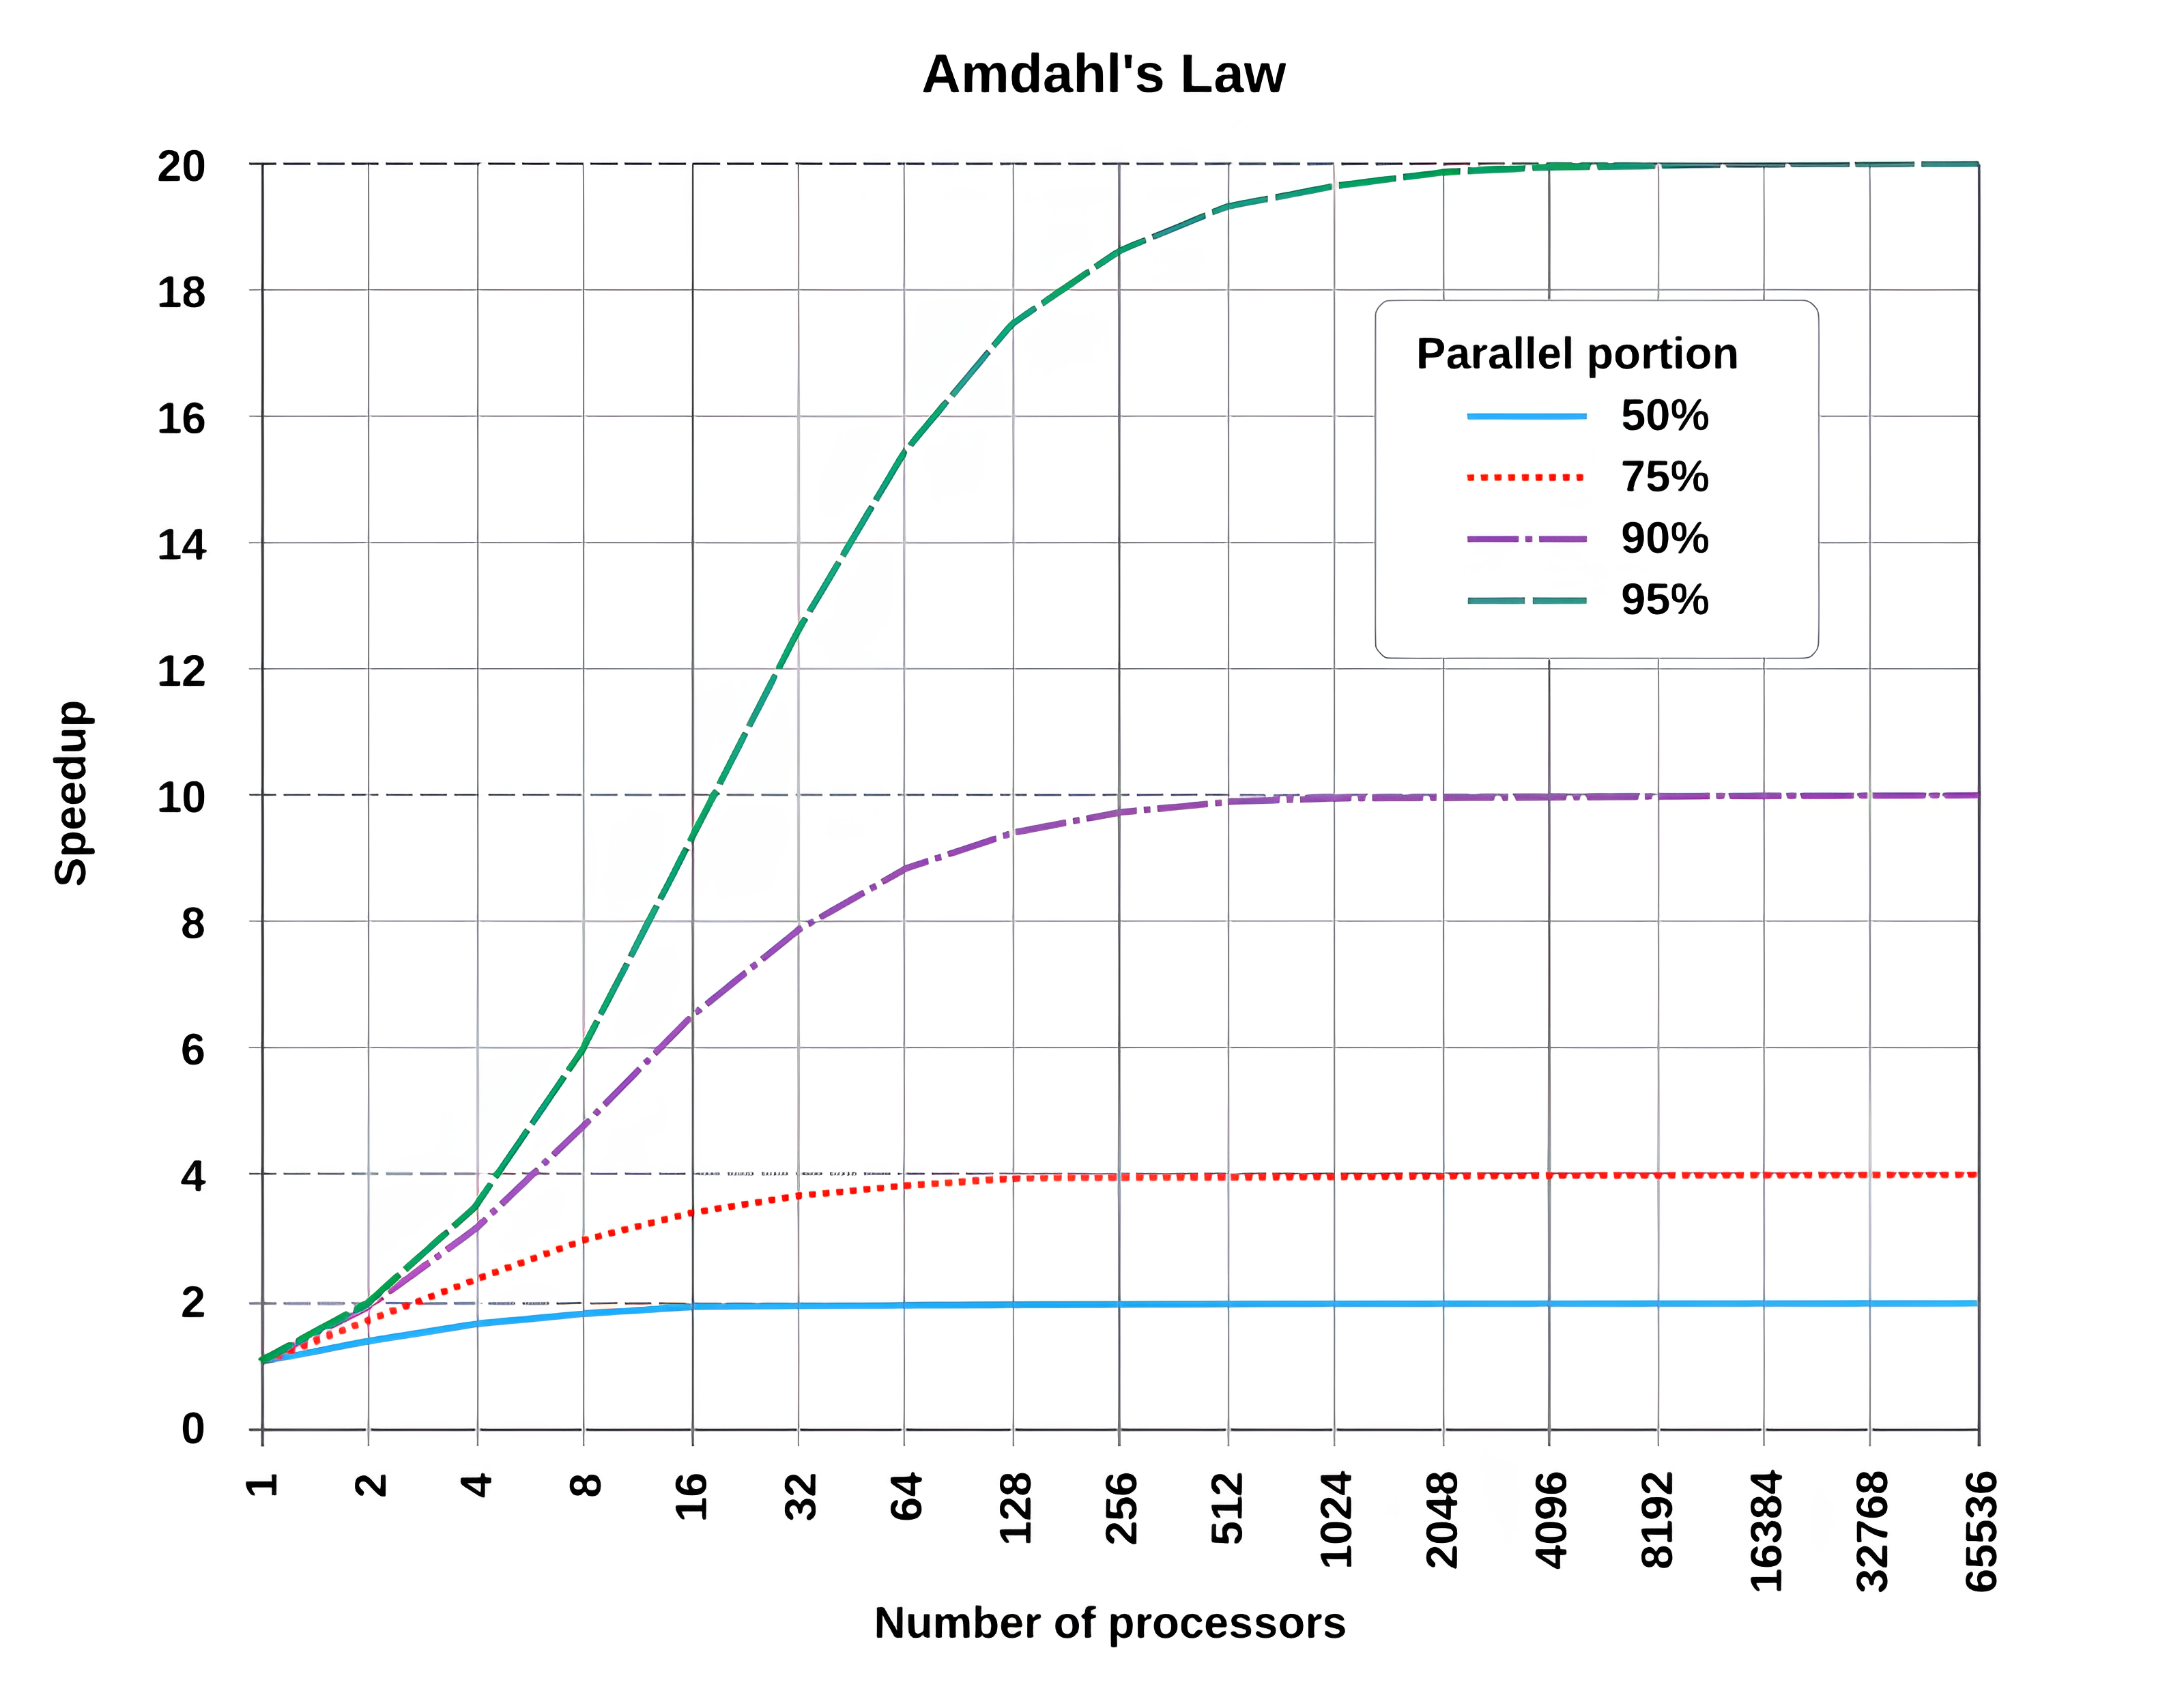
\includegraphics[width=0.7\textwidth]{images/Amdahls.png}
\end{center}
Questa legge non tiene conto del week scaling e decreta un comportamento ideale/approssimato. La \textbf{legge 
di Gustafson} tiene conto del week scaling 
$$ S(n,p)=(1-\alpha)+\alpha p$$
Nel caso reale, l'aumentare del numero di processi potrebbe far incrementare la frazione seriale.\begin{center}
    \includegraphics[width=0.7\textwidth]{images/speedUp.eps}
\end{center}
\flowerLine
\section{Operazioni su Vettori e Matrici}
\subsection{Scatter e Gather}
Consideriamo un algoritmo sequenziale che calcoli la somma di due vettori dati in input 
\begin{lstlisting}[style=CStyle]
void vector_sum(double x[], double y[], double z[], int n){
    for(int i=0; i<n; i++){
        z[i]=x[i]+y[i];
    }
}
\end{lstlisting}
Come si può distribuire tale compito su diversi processi? Si da l'assunzione che i vettori da 
sommare siano stati letti da standard input, quindi sono presenti nella memoria del processo con 
rank 0. Si vuole dividere il vettore equamente fra i diversi processi.\acc 
A tal proposito, esiste la funzione collettiva \code{int MPI\_Scatter}, che si occupa di prendere un 
vettore e di dividerlo equamente fra tutti i processi di un dato comunicatore.\begin{center}
    \includegraphics[width=0.4\textwidth]{images/scatter.eps}
\end{center}
I parametri della funzione sono i seguenti\begin{itemize}
    \item \code{void *send\_buf\_p} il buffer contenente il vettore da dividere
    \item  \code{int send\_count} il numero di elementi da inviare ad ogni processo, non il numero di elementi 
    totali del vettore
    \item  \code{MPI\_Datatype send\_type} il tipo degli elementi del vettore 
    \item  \code{void *recv\_buf\_p} il buffer che conterrà la frazione di vettore ricevuta, per il mittente, può 
    coincidere con il buffer di invio 
    \item  \code{int recv\_count} analogo a \codee{send\_count}
    \item  \code{MPI\_Datatype recv\_type} analogo a codee{send\_type}
    \item  \code{int src\_proc} il rank del processo che condividerà il vettore 
    \item \code{MPI\_Comm comm} il comunicatore in questione
\end{itemize}
La funzione assume che il numero di elementi da condividere sia divisibile per il numero di processi, l'ordine 
di condivisione avviene in base al rank. Il nodo che condivide il vettore può specificare la macro 
\code{MPI\_IN\_PLACE} come buffer di destinazione, e manterrà i valori nel vettore originale.\acc 
La funzione collettiva \code{int MPI\_Gather} è l'inversa della \code{scatter}, ogni nodo definisce un vettore, 
e ne verrà eseguita la concatenazione, per poi essere inviata ad un processo.\begin{center}
    \includegraphics[width=0.4\textwidth]{images/gather.eps}
\end{center}
L'ordine di concatenazione è sempre dato dal rank. I parametri sono pressocché identici alla \code{scatter}\begin{itemize}
    \item \code{void *send\_buf\_p} il buffer contenente il vettore parziale da inviare
    \item  \code{int send\_count} il numero di elementi contenuti nel vettore parziale
    \item  \code{MPI\_Datatype send\_type} il tipo degli elementi del vettore 
    \item  \code{void *recv\_buf\_p} il buffer che conterrà il vettore finale composta dalla concatenazione dei 
    vettori parziali 
    \item  \code{int recv\_count} analogo a \codee{send\_count}
    \item  \code{MPI\_Datatype recv\_type} analogo a codee{send\_type}
    \item  \code{int dest\_proc} il rank del processo che riceverà il vettore
    \item \code{MPI\_Comm comm} il comunicatore in questione
\end{itemize}
\textbf{Esempio di codice} : Il seguente programma, fa si che il processo di rank 0 generi 
due vettori con valori casuali, che verranno divisi fra i vari processi che eseguiranno delle somme parziali, 
trovando sezioni parziali del vettore somma, che verrà poi ri-unito con l'operazione collettiva.
\begin{lstlisting}[style=CStyle]
#include <stdio.h>
#include <stdlib.h>
#include <time.h>
#include <mpi.h>

void print_vector(int n, int *v, char name)
{
    printf("%c = [ ", name);
    for (int i = 0; i < n - 1; i++)
    {
        printf("%d, ", v[i]);
    }
    printf("%d ]\n", v[n - 1]);
}

int main(int argc, char **argv)
{
    MPI_Init(NULL, NULL);

    int my_rank;
    int size;
    int local_size = 3;
    MPI_Comm_size(MPI_COMM_WORLD, &size);

    int local_vector[size];
    int local_vector2[size];
    MPI_Comm_rank(MPI_COMM_WORLD, &my_rank);

    if (my_rank == 0)
    {

        int inputVector[local_size * size];
        int inputVector2[local_size * size];
        srand(time(NULL));
        for (int i = 0; i < local_size * size; i++)
        {
            inputVector[i] = rand() % 100;
            inputVector2[i] = rand() % 100;
        }
        print_vector(local_size * size, inputVector, 'A');
        print_vector(local_size * size, inputVector2, 'B');
        printf("\n");
        MPI_Scatter(inputVector, local_size, MPI_INT, local_vector, local_size,
                     MPI_INT, 0, MPI_COMM_WORLD);
        MPI_Scatter(inputVector2, local_size, MPI_INT, local_vector2, local_size,
                     MPI_INT, 0, MPI_COMM_WORLD);
    }
    else
    {
        MPI_Scatter(NULL, local_size, MPI_INT, local_vector, local_size,
                     MPI_INT, 0, MPI_COMM_WORLD);
        MPI_Scatter(NULL, local_size, MPI_INT, local_vector2, local_size,
                     MPI_INT, 0, MPI_COMM_WORLD);
    }
    printf("process %d :\n     A_%d = [ ", my_rank, my_rank);
    for (int i = 0; i < local_size - 1; i++)
    {
        printf("%d, ", local_vector[i]);
    }
    printf("%d ]\n     B_%d = [", local_vector[local_size - 1], my_rank);
    for (int i = 0; i < local_size - 1; i++)
    {
        printf("%d, ", local_vector2[i]);
    }
    printf("%d ]\n A_%d+B_%d = [", local_vector2[local_size - 1], my_rank, my_rank);
    for (int i = 0; i < local_size - 1; i++)
    {
        printf("%d, ", local_vector2[i] + local_vector[i]);
    }
    printf("%d ]\n\n", local_vector2[local_size - 1] + local_vector[local_size - 1]);

    int vec_sum[local_size];
    for (int i = 0; i < local_size; i++)
    {
        vec_sum[i] = local_vector2[i] + local_vector[i];
    }

    if (my_rank == 0)
    {
        int outVector[local_size * size];
        MPI_Gather(vec_sum, local_size, MPI_INT, outVector, local_size,
                    MPI_INT, 0, MPI_COMM_WORLD);
        print_vector(local_size * size, outVector, 'O');
    }
    else
    {
        MPI_Gather(vec_sum, local_size, MPI_INT, NULL, local_size,
                    MPI_INT, 0, MPI_COMM_WORLD);
    }

    MPI_Finalize();

    exit(0);
}
\end{lstlisting}
Le operazioni collettive sui vettori possono essere eseguite anche sulle matrici, anche se ciò dipende 
dall'allocazione di esse. Quando si dichiara una matrice di dimensioni 
statiche nel seguente modo \begin{quotation}
    \code{int matrix[n][n];}
\end{quotation}
essa viene allocata in maniera contigua in memoria.
\begin{center}
    \includegraphics[width=0.8\textwidth]{images/matrixDeclaration.eps}
\end{center}
In tal caso, le operazioni collettive di \textit{reduce} funzioneranno senza problemi dato che 
agiscono su blocchi di memoria contigui. Il punto è che una dichiarazione di questo tipo ha senso 
esclusivamente se è nota a priori la dimensione della matrice, nel caso più generale, una matrice 
si dichiara dinamicamente come un puntatore di puntatori di interi.
\begin{lstlisting}[style=CStyle]
int** a;
a = (int**) malloc(sizeof(int*)*num_rows);
for(int i = 0; i < num_rows; i++){
    a[i] = (int*) malloc(sizeof(int)*num_cols);
}
\end{lstlisting}
Le righe della matrice in questo caso \textit{non} sono contigue in memoria, non è quindi possibile 
utilizzare operazioni di \textit{reduce}, per far ciò, bisogna collassare la matrice in un 
array bidimensionale regolando l'accesso degli indici. Su una matrice statica, l'accesso avviene 
per mezzo di due indici \code{matrix[i][j]}, se la matrice è collassata in un 
array, un solo indice deve codificare entrambi gli indici della matrice, nella pratica, si fa così\begin{quote}
    \code{matrix[i*num\_col+j]}
\end{quote}
Una matrice allocata dinamicamente come un unico array può essere soggetta alle operazioni di \textit{reduce}.
\begin{center}
    \includegraphics[width=0.8\textwidth]{images/matrixDeclaration2.eps}
\end{center}
\subsubsection{Prodotto fra Vettori e Matrici}
Come visto nel corso di 
\color{blue}\href{https://github.com/CasuFrost/University_notes/blob/main/Secondo%20Anno/Primo%20Semestre/Algebra/Latex%20source%20file/Algebra.pdf}{Algebra}\color{black}, 
il prodotto scalare fra due vettori è definito come segue 
$$ \begin{bmatrix}
    a_1&a_2&\dots&a_n
\end{bmatrix}\cdot \begin{bmatrix}
    b_1\\b_2\\\dots\\b_n
\end{bmatrix}=a_1\cdot b_1 + a_2\cdot b_2+\dots + a_n\cdot b_n$$
Il prodotto fra una matrice $n\times n$ ed un vettore $\bar b$ di $n$ componenti, è un vettore sempre di 
$n$ componenti, di cui ogni $i$-esimo componente è il prodotto scalare fra la $i$-esima riga della matrice 
ed il vettore $\bar b$. 
$$ \begin{bmatrix}
    a_{1_1}&a_{1_2}&\dots&a_{1_n}\\ 
    a_{2_1}&a_{2_2}&\dots&a_{2_n}\\ 
    \vdots & \vdots &\ddots & \vdots\\ 
    a_{n_1}&a_{n_2}&\dots&a_{n_n}
\end{bmatrix}\cdot \begin{bmatrix}
    b_1\\b_2\\\dots\\b_n
\end{bmatrix}=\begin{bmatrix}
    a_{1_1}b_1+a_{1_2}b_2+\dots+a_{1_n}b_n\\
    a_{2_1}b_1+a_{2_2}b_2+\dots+a_{2_n}b_n\\
    \vdots\\
    a_{n_1}b_1+a_{n_2}b_2+\dots+a_{n_n}b_n
\end{bmatrix}$$
\begin{lstlisting}[style=CStyle]
int A[n][n]; //matrice 
int b[n]; //vettore input
int y[n]; //vettore risultato
for(i=0;i<n;i++){
    for(j=0;j<n;j++){
        y[i]=A[i][j]*b[j] //prodotto scalare implicitamente definito
    }
}
\end{lstlisting}








\newpage\subsection{Ultime Collettive di tipo "All"}
\end{document}